\documentclass[aspectratio=169,11pt]{beamer}

% Presentation slides for steady_state_error.tex (the accompanying document has the details)

\usetheme{default}
\setbeamertemplate{navigation symbols}{}
\setbeamertemplate{footline}[frame number]
\setbeamertemplate{itemize items}[circle]
\setbeamerfont{frametitle}{series=\bfseries}

\usepackage{amsmath, amssymb}
\usepackage{booktabs}
\usepackage{tikz}
\usetikzlibrary{arrows.meta, positioning, calc, fit}

\graphicspath{{../../chapter/}}

\tikzset{
  >=Latex, thick,
  block/.style = {draw, rectangle, minimum height=2.2em, minimum width=4em},
  sum/.style   = {draw, circle, inner sep=0pt, minimum size=1.1em},
}

\title{Steady-State Error Analysis}
\subtitle{ME 2801}
\author{}
\date{}

\begin{document}

% ---------------------------------------------------------------------------
\begin{frame}
  \titlepage
  \centering\small Details, derivations and examples: \emph{Steady-State Error Analysis} (notes)
\end{frame}

% ---------------------------------------------------------------------------
\begin{frame}{The question}
  After the transients die out, where does the output settle relative to the reference?

  \bigskip
  \begin{center}
  \begin{tabular}{ll}
    \toprule
    Transient response        & Steady state \\
    \midrule
    Settling time, overshoot  & Final offset, ramp lag \\
    Damping ratio             & Persistent tracking error \\
    Pole locations            & DC behavior of the loop \\
    \bottomrule
  \end{tabular}
  \end{center}

  \bigskip
  Commanded 5\,m/s: does the USV reach 5\,m/s, or settle 0.3\,m/s short?
\end{frame}

% ---------------------------------------------------------------------------
\begin{frame}{Setup: unity negative feedback}
  \begin{center}
  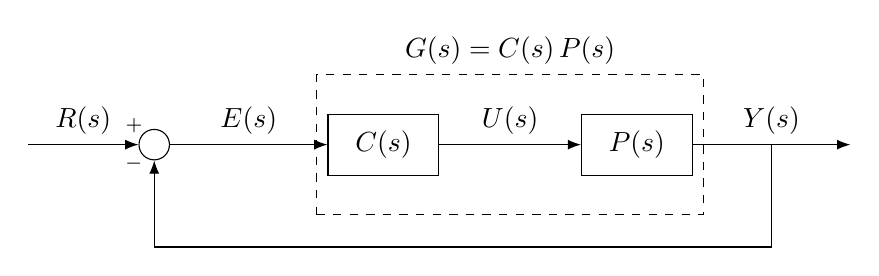
\begin{tikzpicture}
    \node[coordinate]                   (rin)  {};
    \node[sum,   right=1.4cm of rin]    (sum)  {};
    \node[block, right=2.0cm of sum]    (C)    {$C(s)$};
    \node[block, right=1.8cm of C]      (P)    {$P(s)$};
    \node[coordinate, right=2.0cm of P] (yout) {};
    \node[font=\scriptsize, inner sep=0pt, anchor=south east] at (sum.north west) {$+$};
    \node[font=\scriptsize, inner sep=0pt, anchor=north east] at (sum.south west) {$-$};
    \draw[->] (rin) -- node[above]{$R(s)$} (sum);
    \draw[->] (sum) -- node[above]{$E(s)$} (C);
    \draw[->] (C)   -- node[above]{$U(s)$} (P);
    \draw[->] (P)   -- node[above]{$Y(s)$} (yout);
    \coordinate (fbk) at ($(P.east)!0.5!(yout)$);
    \draw[->] (fbk) -- ++(0,-1.3) -| (sum.south);
    \node[draw, dashed, inner xsep=4pt, inner ysep=14pt, fit=(C)(P), label=above:{$G(s) = C(s)\,P(s)$}] {};
  \end{tikzpicture}
  \end{center}

  \begin{itemize}
    \item $G(s)$ is the \emph{combined} open-loop forward path: controller times plant
    \item Error signal: $E(s) = R(s) - Y(s)$
    \item Closed loop must be \emph{stable}, otherwise the final value theorem does not apply
  \end{itemize}
\end{frame}

% ---------------------------------------------------------------------------
\begin{frame}{The master equation}
  From $Y = G E$ and $E = R - Y$:
  \[
    E(s) = \frac{R(s)}{1 + G(s)}
  \]
  Final value theorem: $e(\infty) = \lim_{s\to 0} s\,E(s)$, so
  \[
    \boxed{\,e(\infty) = \lim_{s \to 0} \frac{s\,R(s)}{1 + G(s)}\,}
  \]

  \medskip
  Everything that follows is this formula with a specific $R(s)$ and $G(s)$.
\end{frame}

% ---------------------------------------------------------------------------
\begin{frame}{Three test inputs}
  \begin{center}
  \begin{tabular}{llcc}
    \toprule
    Input    & Scenario                          & $r(t)$           & $R(s)$  \\
    \midrule
    Step     & Hold a new position or speed      & $1$              & $1/s$   \\
    Ramp     & Follow a constant-velocity target & $t$              & $1/s^2$ \\
    Parabola & Follow an accelerating target     & $\tfrac12 t^2$   & $1/s^3$ \\
    \bottomrule
  \end{tabular}
  \end{center}

  \bigskip
  Each harder input needs one more integrator in $G(s)$ to keep the error bounded.
\end{frame}

% ---------------------------------------------------------------------------
\begin{frame}{One formula, three errors}
  \begin{align*}
    e_{\rm step}(\infty) &= \frac{1}{1 + \lim_{s\to 0} G(s)} \\[6pt]
    e_{\rm ramp}(\infty) &= \frac{1}{\lim_{s\to 0} s\,G(s)} \\[6pt]
    e_{\rm para}(\infty) &= \frac{1}{\lim_{s\to 0} s^2 G(s)}
  \end{align*}

  \medskip
  The answer depends on how many poles $G(s)$ has at $s = 0$.
\end{frame}

% ---------------------------------------------------------------------------
\begin{frame}{System type}
  \[
    G(s) = \frac{K\,(s + z_1)(s + z_2)\cdots}{s^n\,(s + p_1)(s + p_2)\cdots}
    \qquad \text{Type } n = \text{number of integrators}
  \]

  \begin{itemize}
    \item A property of $G(s) = C(s)P(s)$, not the plant alone
    \item Adding an integrator to the controller (P $\to$ PI) raises the type by one
  \end{itemize}

  \medskip
  Example, plant $P(s) = 5/(s+5)$:
  \begin{center}
  \begin{tabular}{llcc}
    \toprule
    Controller & $G(s)$ & Type & Step error \\
    \midrule
    P, $K_P = 2$      & $\dfrac{10}{s+5}$                 & 0 & $1/3$ \\[8pt]
    PI, $K_P + K_I/s$ & $\dfrac{5(K_P s + K_I)}{s(s+5)}$ & 1 & $0$ \\[4pt]
    \bottomrule
  \end{tabular}
  \end{center}
\end{frame}

% ---------------------------------------------------------------------------
\begin{frame}{Static error constants}
  \begin{columns}[T]
    \column{0.42\textwidth}
    \begin{align*}
      K_x &= \lim_{s\to 0} G(s)      & e_{\rm step} &= \frac{1}{1+K_x} \\[4pt]
      K_v &= \lim_{s\to 0} s\,G(s)   & e_{\rm ramp} &= \frac{1}{K_v} \\[4pt]
      K_a &= \lim_{s\to 0} s^2 G(s)  & e_{\rm para} &= \frac{1}{K_a}
    \end{align*}

    \column{0.52\textwidth}
    \centering
    \begin{tabular}{lccc}
      \toprule
      Input    & Type 0          & Type 1          & Type 2 \\
      \midrule
      Step     & $\dfrac{1}{1+K_x}$ & $0$             & $0$ \\[8pt]
      Ramp     & $\infty$            & $\dfrac{1}{K_v}$ & $0$ \\[8pt]
      Parabola & $\infty$            & $\infty$         & $\dfrac{1}{K_a}$ \\[4pt]
      \bottomrule
    \end{tabular}
  \end{columns}

  \bigskip
  Type $n$: zero error for simpler inputs, finite for input $n$, infinite for harder inputs.
\end{frame}

% ---------------------------------------------------------------------------
\begin{frame}{Type 0 vs.\ Type 1: step and ramp}
  \begin{columns}[c]
    \column{0.5\textwidth}
    \centering
    \includegraphics[width=\linewidth,height=0.72\textheight,keepaspectratio]{images/sse_step_compare.pdf}\\
    \small Step: Type 0 settles short; Type 1 tracks exactly

    \column{0.5\textwidth}
    \centering
    \includegraphics[width=\linewidth,height=0.72\textheight,keepaspectratio]{images/sse_ramp_compare.pdf}\\
    \small Ramp: Type 0 diverges, Type 1 lags by $1/K_v$, Type 2 tracks
  \end{columns}
\end{frame}

% ---------------------------------------------------------------------------
\begin{frame}{Reading an error specification}
  Given the spec $K_v = 20$, we can conclude:
  \begin{enumerate}
    \item The system is stable (otherwise the spec is undefined)
    \item The system is Type 1 (only Type 1 has a finite, nonzero $K_v$)
    \item The relevant test input is a ramp
    \item The ramp error per unit slope is $1/K_v = 0.05 = 5\%$
  \end{enumerate}
\end{frame}

% ---------------------------------------------------------------------------
\begin{frame}{Design: choose the gain to meet a spec}
  \begin{columns}[T]
    \column{0.5\textwidth}
    $G(s) = \dfrac{K(s+3)}{s(s+6)(s+10)}$

    \smallskip
    Want a 5\% ramp error.

    \medskip
    \begin{enumerate}
      \item Type 1 $\Rightarrow$ finite ramp error
      \item $K_v = \lim_{s\to 0} s\,G(s) = \dfrac{3K}{60} = \dfrac{K}{20}$
      \item $1/K_v = 0.05 \Rightarrow K_v = 20 \Rightarrow \boxed{K = 400}$
    \end{enumerate}

    \column{0.5\textwidth}
    \centering
    \includegraphics[width=\linewidth,height=0.7\textheight,keepaspectratio]{images/sse_design.pdf}
  \end{columns}
\end{frame}

% ---------------------------------------------------------------------------
\begin{frame}{Why an integrator removes step error}
  \begin{columns}[T]
    \column{0.48\textwidth}
    $u_I(t) = K_I \int_0^t e(\tau)\,d\tau \quad\Rightarrow\quad \dot u_I = K_I\,e$

    \medskip
    \begin{itemize}
      \item At steady state every signal is constant, so $\dot u_I = 0$
      \item That requires $e = 0$
      \item The integrator keeps adjusting until the error is gone, whatever the cause: drag, wind, current
    \end{itemize}

    \column{0.5\textwidth}
    \centering
    \includegraphics[width=\linewidth,height=0.75\textheight,keepaspectratio]{images/sse_integrator_adapt.pdf}
  \end{columns}
\end{frame}

% ---------------------------------------------------------------------------
\begin{frame}{Integral action is not free}
  \begin{itemize}
    \item \textbf{Higher closed-loop order:} a first-order plant with PI becomes second order and can overshoot
    \item \textbf{Windup:} while the actuator saturates, the integrator keeps charging and then drives overshoot
    \item \textbf{Harder to stabilize:} each integrator reduces stability margin (frequency response, later)
  \end{itemize}
\end{frame}

% ---------------------------------------------------------------------------
\begin{frame}{Feedforward: the other way to remove step error}
  \begin{center}
  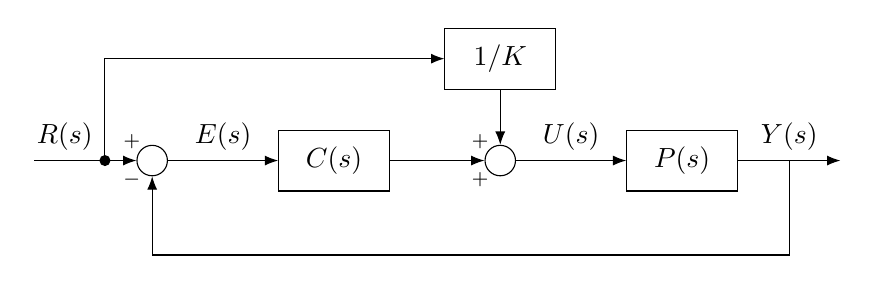
\begin{tikzpicture}
    \node[coordinate]                   (rin)  {};
    \node[sum,   right=1.3cm of rin]    (esum) {};
    \node[block, right=1.4cm of esum]   (C)    {$C(s)$};
    \node[sum,   right=1.2cm of C]      (usum) {};
    \node[block, right=1.4cm of usum]   (P)    {$P(s)$};
    \node[coordinate, right=1.3cm of P] (yout) {};
    \node[block, above=0.7cm of usum]   (FF)   {$1/K$};
    \node[font=\scriptsize, inner sep=0pt, anchor=south east] at (esum.north west) {$+$};
    \node[font=\scriptsize, inner sep=0pt, anchor=north east] at (esum.south west) {$-$};
    \node[font=\scriptsize, inner sep=0pt, anchor=north east] at (usum.south west) {$+$};
    \node[font=\scriptsize, inner sep=0pt, anchor=south east] at (usum.north west) {$+$};
    \coordinate (rb) at ($(rin)!0.6!(esum)$);
    \fill (rb) circle (2pt);
    \draw[->] (rin)  -- node[above, pos=0.3]{$R(s)$} (esum);
    \draw[->] (rb)   |- (FF);
    \draw[->] (FF)   -- (usum.north);
    \draw[->] (esum) -- node[above]{$E(s)$} (C);
    \draw[->] (C)    -- (usum);
    \draw[->] (usum) -- node[above]{$U(s)$} (P);
    \draw[->] (P)    -- node[above]{$Y(s)$} (yout);
    \coordinate (fbk) at ($(P.east)!0.5!(yout)$);
    \draw[->] (fbk) -- ++(0,-1.2) -| (esum.south);
  \end{tikzpicture}
  \end{center}

  \begin{itemize}
    \item Supplies the steady-state effort $r/K$ immediately; output settles at $K \cdot r/K = r$
    \item Relies on knowing the plant DC gain $K$; a wrong $K$ leaves a residual error
    \item Does not change $G(s)$ or the system type, so the master equation does not capture it
  \end{itemize}
\end{frame}

% ---------------------------------------------------------------------------
\begin{frame}{Integrator vs.\ feedforward}
  \begin{columns}[c]
    \column{0.52\textwidth}
    \small
    \begin{tabular}{@{}lll@{}}
      \toprule
                    & Integral          & Feedforward \\
      \midrule
      Model needed  & No                & Plant DC gain \\[3pt]
      Transient     & Slower; overshoot & Fast \\[3pt]
      System type   & $+1$              & Unchanged \\[3pt]
      Disturbances  & Rejects them      & Does not \\
      \bottomrule
    \end{tabular}

    \medskip
    \normalsize
    In practice: PI + feedforward.  Feedforward for speed, integrator for robustness.

    \column{0.46\textwidth}
    \centering
    \includegraphics[width=\linewidth,height=0.75\textheight,keepaspectratio]{images/sse_ff_compare.pdf}
  \end{columns}
\end{frame}

% ---------------------------------------------------------------------------
\begin{frame}{Takeaways}
  \begin{itemize}
    \item One formula: $e(\infty) = \lim_{s\to 0} s\,R(s)/\bigl(1 + G(s)\bigr)$, valid for a stable closed loop
    \item System type (integrators in $G = CP$) sets which inputs give zero, finite or infinite error
    \item Error constants $K_x$, $K_v$, $K_a$ turn a spec into a gain requirement
    \item An integrator removes step error by adapting; feedforward removes it by knowing the plant
    \item Combine them: feedforward for speed, integrator for robustness
  \end{itemize}
\end{frame}

\end{document}
